\subsubsection{Używanie Helpful Sets w celu zmniejszenia długości granic}
Heurystyka Helpful Sets startuje od początkowego podziału i za pomocą lokalnie wprowadzanych zmian zmniejsza długość granic.
Algorytm startuje od poszukiwania zbioru \texttt{k-helpful}, to jest podzbioru wierzchołków ze zbioru $V_1$ lub $V_2$,
który zmniejsza długość granicy o $k$, jeśli zostanie przeniesiony do drugiej partycji.
Jeśli taki zbiór zostaje znaleziony w jednej z dwóch
partycji, na przykład w $V_1$, to jest przenoszony do $V_2$.
Następnie algorytm zaczyna szukać w części $V_2$, która
jest aktualnie wystarczająco duża, aby zbalansować podział i zwiększyć długość granicy o maksymalnie $(k-1)$ krawędzi.
Jeśli taki \texttt{balancing set} zostaje znaleziony, to przenoszony jest do zbioru $V_1$ i proces zaczyna się od początku.
Działanie algorytmu dobrze widać na rysunku \ref{im:balancing} oraz \ref{im:h_steps}.
Zanim algorytm zostanie opisany dokładniej, potrzebne są definicje zbiorów helpful oraz balancing:

\begin{definition}
(diff-value wierzchołka)\newline
Dla wierzchołka $v \subset V$ wartość diff-value definiujemy jako $diff(v) = ext(v) - int(v)$.
\end{definition}

\begin{definition}
(Helpful Set)\newline
Niech $S \subset V_i, i \in \{1,2\}$ będzie podzbiorem wierzchołków partycji. Dla każdego $v \in S$ definiujemy
$int_s(v) = |\{w \in S; \{v,w\} \in E\}|$ - zbiór krawędzi wewnętrznych $S$.

\begin{equation}
H(S)=\sum_{v \in S}(ext(v) - int(v) + int_s(v))
\label{eq:helpful_set2}
\end{equation}
to \textbf{helpfulness} zbioru S. Zbiór S nazywany jest H(S)-\textbf{helpful}.
\end{definition}

Przeniesienie zbioru $S$ do drugiej partycji zmniejsza długość granicy o $H(S)$.
Przykłady zbiorów $2$-helpful pokazane są na rysunku \ref{im:helpfulsets:example}.

Autorzy artykułu \cite{article} zamienne używają pojęć diff-value oraz helpfulness.
W niniejszej pracy używana jest nazwa helpfulness zarówno dla wierzchołków, jak i dla zbiorów.

\begin{figure}[h]
\centering
\begin{subfigure}{.3\textwidth}
    \centering
    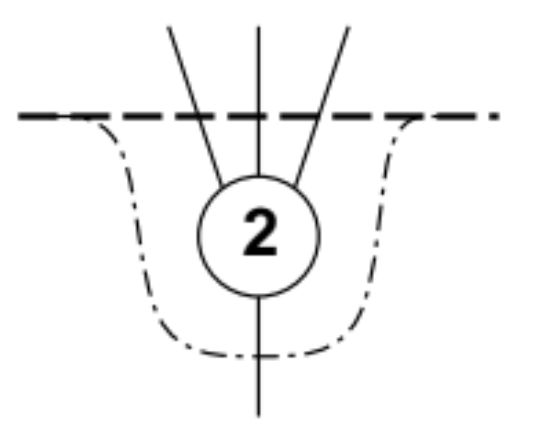
\includegraphics[width=0.55\textwidth]{images/helpfulsets/1}
    \caption[short]{}
\end{subfigure}
\begin{subfigure}{.69\textwidth}
    \centering
    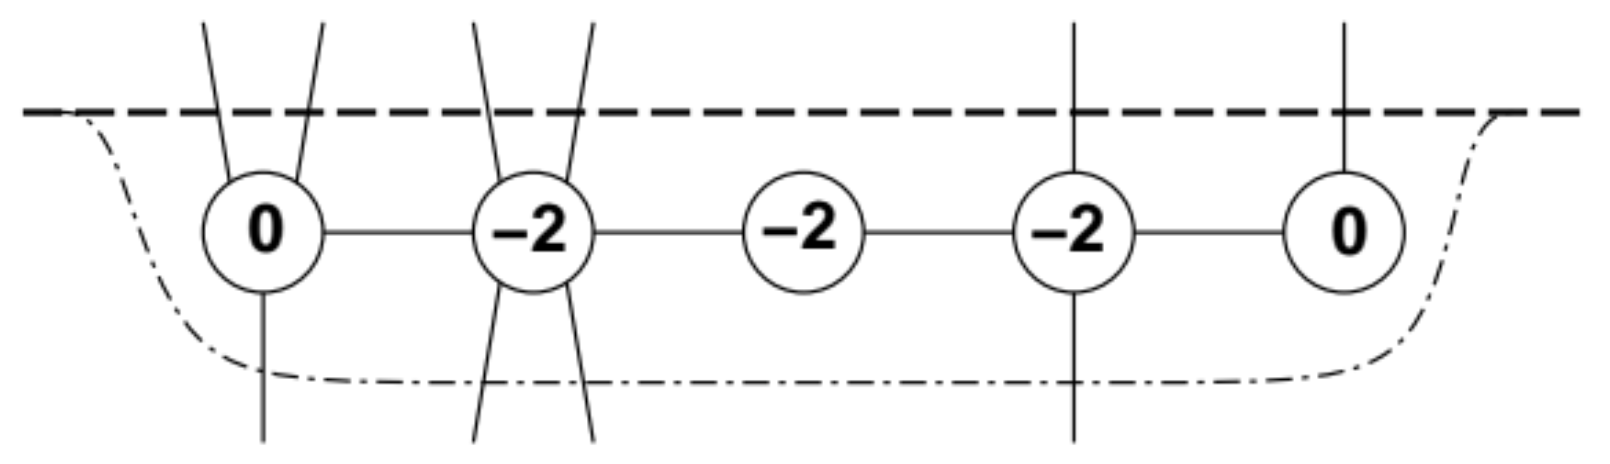
\includegraphics[width=0.68\textwidth]{images/helpfulsets/2}
    \caption[short]{}
\end{subfigure}%

\begin{subfigure}{.4\textwidth}
    \centering
    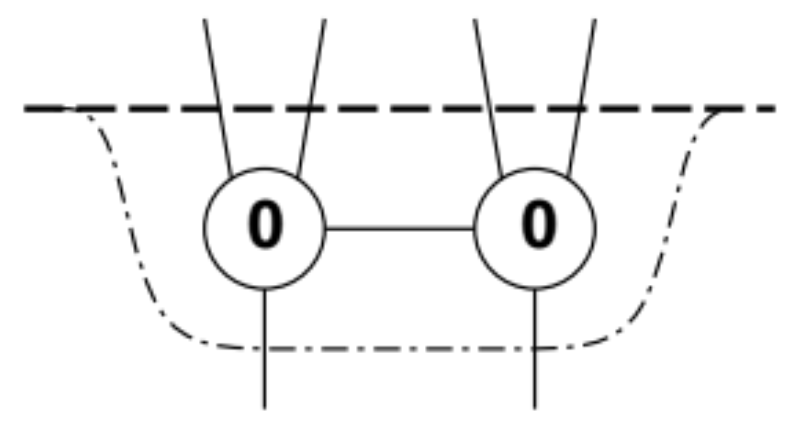
\includegraphics[width=0.63\textwidth]{images/helpfulsets/3}
    \caption[short]{}
\end{subfigure}
\begin{subfigure}{.59\textwidth}
    \centering
    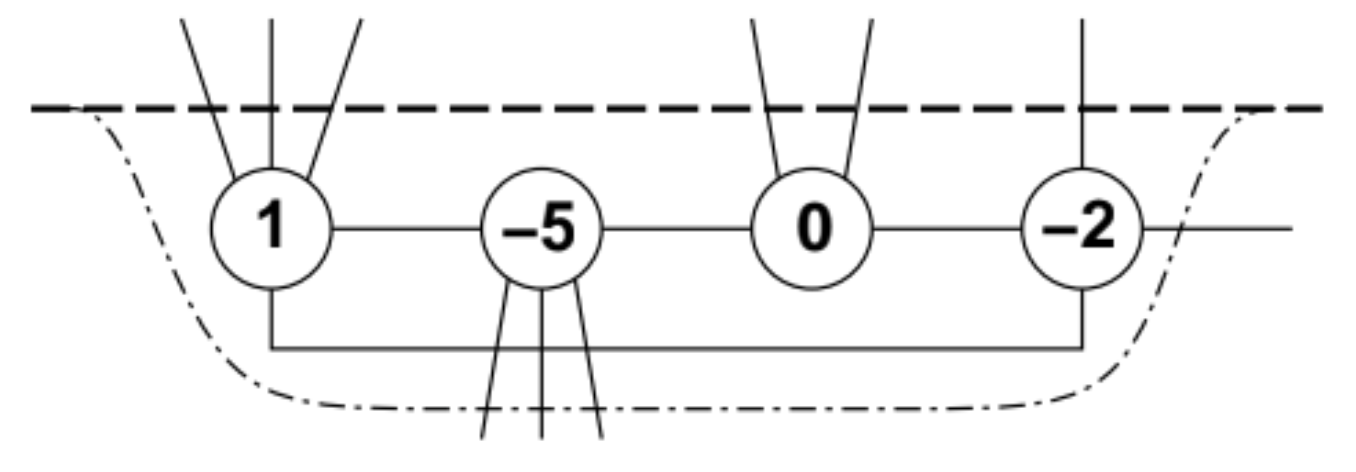
\includegraphics[width=0.68\textwidth]{images/helpfulsets/4}
    \caption[short]{}
\end{subfigure}
\caption{Zbiory 2-helpful. Na górze każdego z 4 przykładów jest zbiór zewnętrzny (ang. external set). Wyliczanie wartości
helpfulness na podstawie wzoru \ref{eq:helpful_set2}: (a): $3-1+0=2$, (b): $6-8+4=2$, (c): $4-3+1=2$ oraz (d): $6-8+4=2$.
Na każdym wierzchołku zaznaczona jest jego wartość helpfuless.
Źródło: \cite{article}.}
\label{im:helpfulsets:example}
\end{figure}

\newpage

\begin{definition}
(Balancing Set)\newline
Niech $S \in V_i$ będzie zbiorem k-helpful. Zbiór $\bar{S} \subset V_j \cup S$, $J \neq i$ nazywany jest \textbf{balancing set}
zbioru S jeśli $|\bar{S}| = |S|$ and $\bar{S}$ jest przynajmniej (-k+1)-helpful.
\end{definition}

Jedną z cech algorytmu jest, że długość granicy zwiększa się o nie więcej niż $(k-1)$ jeśli zbiór $\bar{S}$ przenoszony jest
z jednej partycji do drugiej.


\newcommand\imgss{0.43}

\begin{figure}[h]
\begin{subfigure}{\textwidth}
    \centering
    \fbox{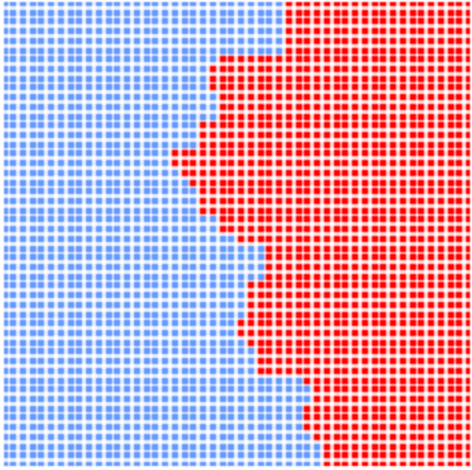
\includegraphics[width=0.215\textwidth]{images/helpful-balancing/1}}
    \caption[short]{początkowy podział}
\end{subfigure}%

\begin{subfigure}{.5\textwidth}
    \centering
    \fbox{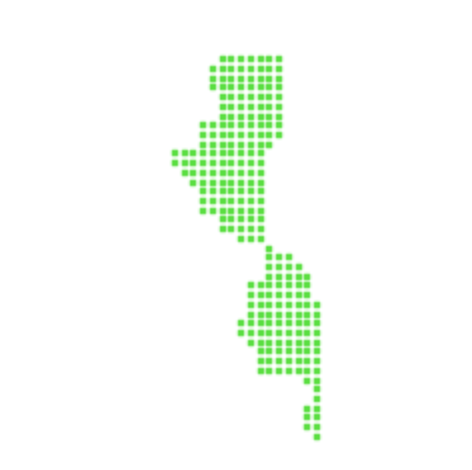
\includegraphics[width=\imgss\textwidth]{images/helpful-balancing/2}}
    \caption[short]{krok 1 - budowanie zbioru helpful}
\end{subfigure}
\begin{subfigure}{.5\textwidth}
    \centering
    \fbox{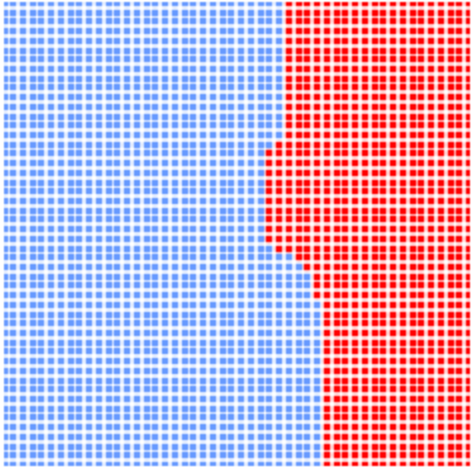
\includegraphics[width=\imgss\textwidth]{images/helpful-balancing/3}}
    \caption[short]{krok 2 - przeniesienie zbioru helpful}
\end{subfigure}%

\begin{subfigure}{.5\textwidth}
    \centering
    \fbox{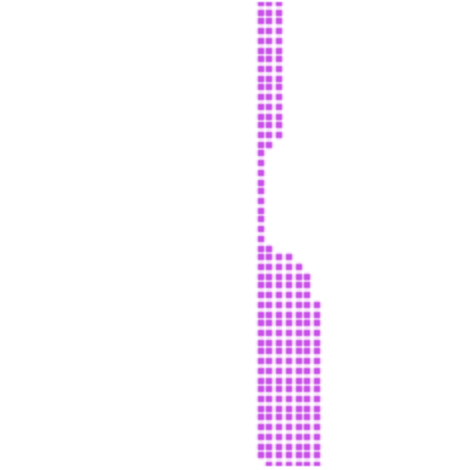
\includegraphics[width=\imgss\textwidth]{images/helpful-balancing/4}}
    \caption[short]{krok 3 - budowanie zbioru balancing}
\end{subfigure}
\begin{subfigure}{.5\textwidth}
    \centering
    \fbox{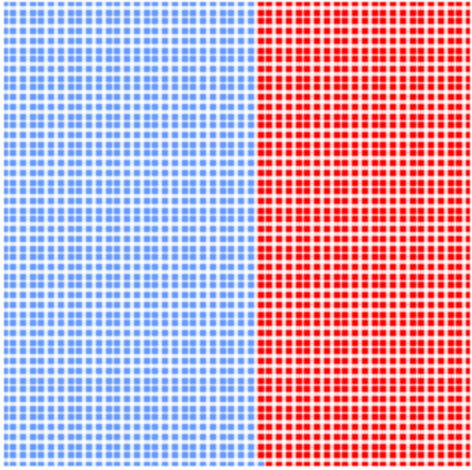
\includegraphics[width=\imgss\textwidth]{images/helpful-balancing/5}}
    \caption[short]{krok 4 - przeniesienie zbioru balancing}
\end{subfigure}%
\caption{Obrazki pokazują początkowy podział, a następnie jedno wywołanie algorytmu Helpful Sets. Rozmiar partycji pozostaje
niemal identyczny, zmniejsza się długość granicy.}
\label{im:balancing}
\end{figure}

\newpage

\begin{pseudocode}
@\underline{HelpfulSet$(A,B)$}@
  IF cut_size$_{A-B}$ $<$ $0$
    RETURN;
  ENDIF
  $l_A \leftarrow l_B \leftarrow cut/2$;                        /* Initialize the limits */
  $s_{max} = (|A| + |B|) / 2) \cdot 0.2$;                /* Initialize max size of HS */
  WHILE $l_A + l_B \geq 1$
    IF $l_A = 0$ OR $2 \cdot l_A \leq l_B$  /* Choose the more promising partition */
      Swap$(A,B)$;
    $S_A$ $=$ BuildHS$(A, l_A, s_{max})$;
    ENDIF
    IF $h(S_A) \leq l_A$ /* If the helpfulness of $S_A$ is smaller than wanted ...
      $l_A \leftarrow b(S_A)$;          ... adjust the limit for the next search */
      IF $l_B > h(S_A)$
        $S_B$ $=$ BuildHS$(B, l_B, s_{max})$;
        IF $h(S_B) \geq h(S_A)$ /* Name the partition with the better set A ...
          Swap$(A, B)$;
        ELSE
          $l_B \leftarrow b(S_B)$; ... and reduce the limit of the other partition */
        ENDIF
      ENDIF
      UndoBuild$(S_B)$;
    ENDIF
    IF $len(S_A) == 0$
      $l_A = 0$;
      CONTINUE;
    ENDIF
    $l_A \leftarrow min(l_A,h(S_A))$;          /* Adjust the limit for the next search */
    MoveSet$(S_A)$                             /* Move the helpful set */
    $min, max$ $\leftarrow$ DetermineMaxAndMin$(w(S_A))$;
    $S_B$ $=$ BuildBS$(B,1 - h(S_A),min,max)$;
    IF $w_l \leq w(S_B) \leq w_h$ and $h(S_B) > -h(S_A)$  /* Check, if the BS is ok */
      MoveSet$(S_B)$;                       /* Yes: Move the BS */
      $l_A \leftarrow l_A + \log(l_A)$;                  /* Increase the limits */
      $l_B \leftarrow l_B + 1$;
    ELSE
      UndoBuild$(S_B)$;           /* No: Undo the build operation and
      UndoMove$(S_A)$;              the movement of the helpful set */
      $l_A \leftarrow l_A/4$;                            /* Reduce the limits */
      $l_B \leftarrow l_B/2$;
    ENDIF
  ENDWHILE
  IF cut_size$_{A-B}$ $>$ $0.1$ $\cdot$ longer_edge_of_a_grid
    Balance$(A, B)$;
  ENDIF
\end{pseudocode}
\vspace{-8mm}
\captionof{listing}{Kod przedstawiający zmodyfikowany na potrzeby niniejszej pracy algorytm Helpful-Set $2$-partitioning.}
\label{code:helpful_sets}
\newpage
Kluczowym elementem algorytmu jest ustalenie wartości helpfulness $l$ zbiorów, których szukamy.
Jeśli wartość $l$ jest zbyt mała, to obiecujące zbiory są przeoczane, natomiast jeśli $l$ jest za duże,
to czas wykonywania algorytmu jest dłuższy, natomiast znalezione przy tym zbiory nie są lepsze.
W celu uzyskania $l$, Party używa techniki zwanej \texttt{adaptive limitation} \cite{article}.
Początkowe $l$ ustawiane jest na wartość $cut/2$.
Wartość $l$ jest zmniejszana o połowę albo ustawiana na najlepszą znalezioną wartość helpfulness, jeśli zbiór $l$-helpful
nie może zostać znaleziony w żadnym z dwóch optymalizowanych zbiorów oraz podwajana, jeśli poszukiwanie
zakończy się sukcesem.
Autorzy \cite{1364754} zaproponowali kilka modyfikacji do algorytmu.
Po pierwsze, zamiast używać pojedynczego limitu $l$ użyto dwóch oddzielnych limitów dla zbioru $A$ oraz zbioru $B$.
Po drugie, dopuszczono do pojawiania się małych różnic wielkości obszarów.
Jest to szczególnie ważne, kiedy podział optymalizowany jest wielokrotnie, na niecałkowicie przywróconym
do początkowego rozmiaru grafie.
Przenoszone wówczas wierzchołki mają często wagi $\geq 1$, ponadto istnieją różnice pomiędzy wagami wierzchołków,
co przekłada się na trudności w idealnym zbalansowaniu optymalizowanych obszarów.
To podejście zostało również zaimplementowane w bibliotekach Jostle and Metis.
Udowodniono, że wpływa ono pozytywnie na optymalizację długości granic, ponieważ dopuszczenie niewielkich
różnic w powierzchni pól pozwala zwykle na lepsze zoptymalizowanie długości granic.
Po trzecie algorytm balansowania obszarów, który zachłannie wyrównuje pola obszarów został przeniesiony na koniec.

Algorytm \ref{code:helpful_sets} przedstawia zmodyfikowaną przeze mnie procedurę.
Pierwszą moją modyfikacją jest sprawdzanie, czy balansowane obszary wciąż ze sobą graniczą (linia $2$).
Może się zdarzyć, że na skutek balansowania innych obszarów granica ta zostanie przerwana.
Jak w poprzedniej implementacji, limity $l_A$ oraz $l_B$ ustawiane są na połowę aktualnej długości granicy pomiędzy
obszarami $A$ i $B$ (linia $5$).
W rozwiązaniu zaproponowanym przez autorów \cite{1364754}, podczas wyszukiwania, wartość helpful zbioru helpful nie może stać się mniejsza
niż $-d/2$, nie może również przekroczyć wagi $s_{max}$.
Wartość $d$ to średni stopień wierzchołka w grafie.
Dla mojej implementacji mógłbym założyć, że $d$ jest zawsze równe $4$ - wynika to ze sposobu, w jaki buduję
graf z wejściowej siatki (rysunek \ref{im:indivisible}).
Jednak ta zasada nie działa.
Algorytm budowania zbioru helpful jest bowiem zachłanny i często budował zbiory, które spełniały kryterium nieprzekraczania
wagi $s_{max}$ oraz miały ujemną wartość helpful, większą niż $-2$.
W kodzie oryginalnego algorytmu później sprawdzane było, czy zbiór nie ma ujemnej wartości helpful i
jeśli miał to budowanie zaczynało się od początku.
Przez to algorytm wywoływał się wielokrotnie bez zakończenia się sukcesem.
Moim rozwiązaniem była zmiana tej instrukcji na warunek na wielkość zbioru $S_A$ (linia $25$) oraz na
pozwolenie na budowanie zbiorów o wartości helpful większej bądź równej $0$ (linia $11$ oraz $16$).
$s_{max}$ z kolei, autorzy \cite{article} ustawiali na wartość $128$.
Ja uzależniłem $s_{max}$ od rozmiaru optymalizowanych partycji (linia $6$).
Użyty do tego współczynnik $0.2$ może zostać dowolnie zmieniony.
Jednak wedle mojego doświadczenia powinien być on raczej mniejszy niż $0.4$, aby zbiór helpful nie był zbyt duży.
Zwiększa to czas partycjonowania, ale nie poprawia wyników.
Lepiej by był on nieco za mały niż za duży, ponieważ po udanych znalezieniu małego zbioru helpful oraz zbioru balancig
limit i tak zostanie zwiększony, a zaczynanie od bardzo dużego zbioru helpful często kończy się nieudanym poszukiwaniem
zbioru balancing i powrotem do początkowego podziału.
Poszukiwanie dużego zbioru jest bardziej kosztowne.

\newpage
\begin{figure}[h]
\begin{subfigure}{\textwidth}
    \centering
    \fbox{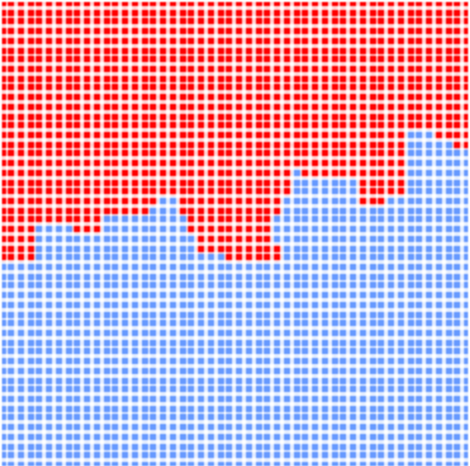
\includegraphics[width=0.215\textwidth]{images/helpfulsets-sh/0}}
    \caption[short]{początkowy podział}
\end{subfigure}%

\begin{subfigure}{.5\textwidth}
    \centering
    \fbox{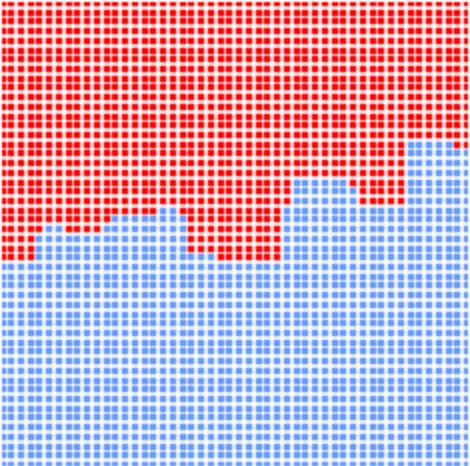
\includegraphics[width=\imgss\textwidth]{images/helpfulsets-sh/1}}
    \caption[short]{krok 1 - przeniesienie zbioru helpful}
\end{subfigure}
\begin{subfigure}{.5\textwidth}
    \centering
    \fbox{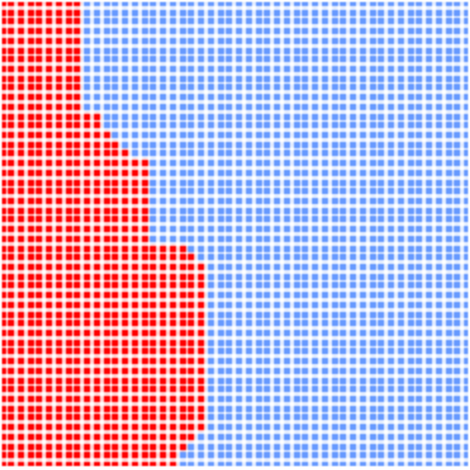
\includegraphics[width=\imgss\textwidth]{images/helpfulsets-sh/2}}
    \caption[short]{krok 2 - przeniesienie zbioru balancing}
\end{subfigure}%

\begin{subfigure}{.5\textwidth}
    \centering
    \fbox{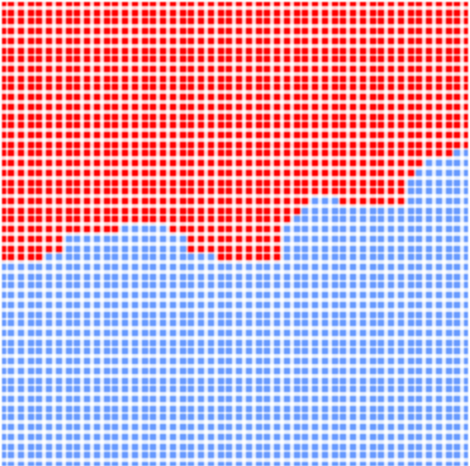
\includegraphics[width=\imgss\textwidth]{images/helpfulsets-sh/3}}
    \caption[short]{krok 3 - przeniesienie zbioru helpful}
\end{subfigure}
\begin{subfigure}{.5\textwidth}
    \centering
    \fbox{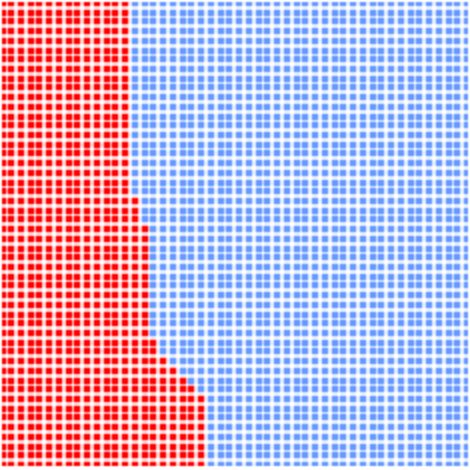
\includegraphics[width=\imgss\textwidth]{images/helpfulsets-sh/4}}
    \caption[short]{krok 4 - przeniesienie zbioru balancing}
\end{subfigure}%

\begin{subfigure}{.5\textwidth}
    \centering
    \fbox{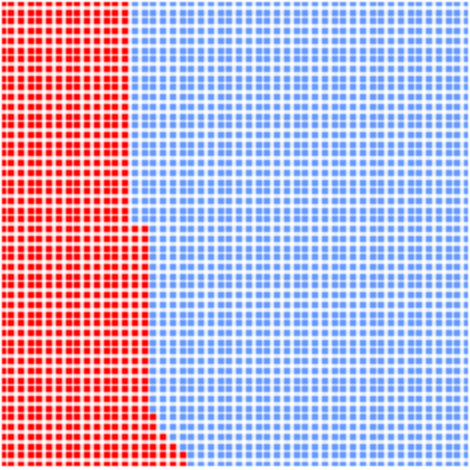
\includegraphics[width=\imgss\textwidth]{images/helpfulsets-sh/5}}
    \caption[short]{krok 5 - przeniesienie zbioru helpful}
\end{subfigure}
\begin{subfigure}{.5\textwidth}
    \centering
    \fbox{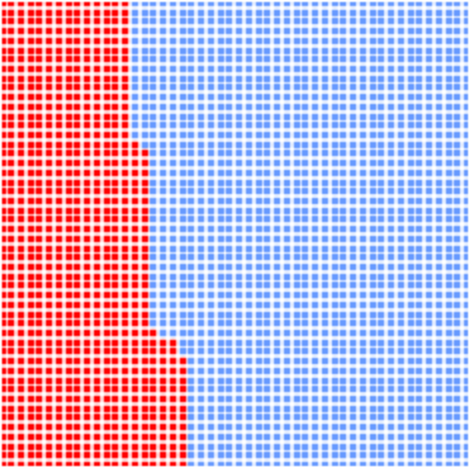
\includegraphics[width=\imgss\textwidth]{images/helpfulsets-sh/6}}
    \caption[short]{krok 6 - przeniesienie zbioru balancing}
\end{subfigure}%

\begin{subfigure}{.5\textwidth}
    \centering
    \fbox{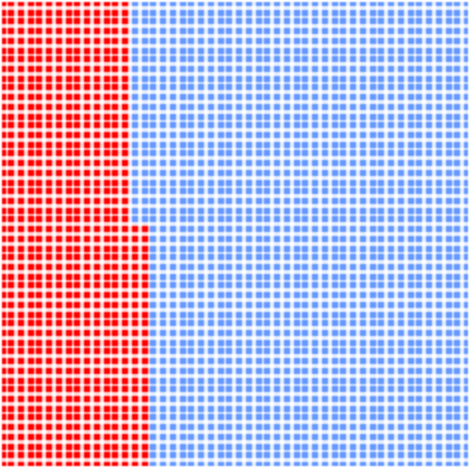
\includegraphics[width=\imgss\textwidth]{images/helpfulsets-sh/7}}
    \caption[short]{krok 7 - przeniesienie zbioru helpful}
\end{subfigure}
\begin{subfigure}{.5\textwidth}
    \centering
    \fbox{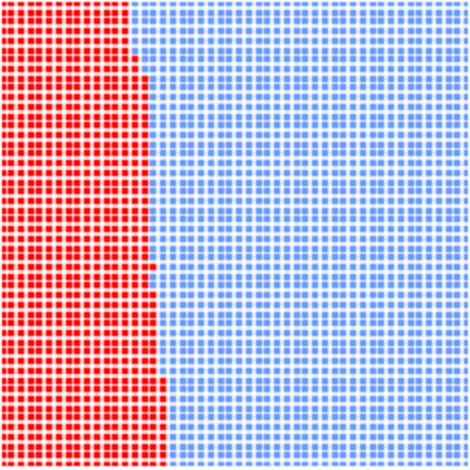
\includegraphics[width=\imgss\textwidth]{images/helpfulsets-sh/8}}
    \caption[short]{krok 8 - przeniesienie zbioru balancing}
\end{subfigure}
\caption{Obrazki przedstawiają kolejne kroki działania algorytmu Helpful Sets na siatce 50x50 podzielonej na 2 obszary
przez algorytm LAM. W pierszym kroku tworzony jest stosunkowo mały zbiór helpful, a w kolejnym kroku odpowiednio mały zbiór balancing.
W momencie kiedy to się udaje algorytm zwiększa limit liczby wierzchołków, dlatego kolejne kroki wnoszą więcej zmian.
Po 4 cyklach budowania i przenoszenia zbioru helpful oraz zbioru balancing granica między obszarami jest znacząco mniejsza, a wielkość obszarów
zachowana. Na potrzeby przykładu balansowanie pól jest wyłączone.}
\label{im:h_steps}
\end{figure}
\FloatBarrier

Pętla WHILE, która znajduje się między liniami $7$ i $42$ jest wykonywana, dopóki suma limitów jest większa od $1$.
W oryginalnej implementacji było to $0$, jednak wedle mojego doświadczenia algorytm wywoływał się wtedy bardzo długo,
niekoniecznie zwiększając jakość partycjonowania.
Jeśli zbiór $l_A$-helpful ($S_A$) (z wagą $w(S_A)$ oraz wartością helpfulness wynoszącą $h(S_A)$) nie może zostać
znaleziony (linia $12$), limit jest redukowany to najlepszej znalezionej wartości helpfulness ($b(S_A)$).
Dalej podejmowana jest decyzja czy nastąpi wyszukiwanie w partycji $B$ (linia $14$).
Jeśli limit $l_A$ jest dużo mniejszy od limitu $l_B$ zbiory $A$ i $B$ są ze sobą zamieniane.
Ten warunek powoduje, że zbiór helpful szukany jest najpierw w bardziej obiecującej partycji.
Jeśli tak, to ustalany jest zbiór $S_B$ (linia $15$).
Dalej zbiór z większą wartością helpfulness jest nazywany $S_A$ (linia $17$) lub limit
drugiej partycji jest redukowany (linia $19$), a zbiór $S_B$ usuwany (linia $22$).
Jeśli wielkość zbioru helpful jest równa $0$, to limit ustawiany jest na $0$ (linia $25$), a algorytm powtarzany.
W przeciwnym wypadku do $l_A$ przypisywana jest nowa wartość (linia $28$), $S_A$ przenoszone jest do $B$ (linia $29$),
a wywołanie wkracza w fazę szukania zbioru balancing.
W tym celu obliczany jest przedział $[min, max]$ dla zbioru balancing (linia $30$).
W implementacji zaproponowanej w \cite{1364754} wartości $min$ oraz $max$ były obliczane w następujący sposób:
\vspace{-3mm}
\begin{pseudocode}
$min \leftarrow (w(B) - w_{max}(B) - grace)^+$
$max \leftarrow (w(B) - w_{min}(B) + grace)^+$
\end{pseudocode}
\vspace{-13mm}
\captionof{listing}{}
\label{code:old_min_max}
\vspace{3mm}
gdzie $grace$ jest połową wagi najcięższego wierzchołka.
Jednak ten sposób wyznaczania wartości $min$ oraz $max$ nie sprawdzał się w moich testach.
$max$ i $min$ pozwalają na budowanie zbioru balancing o przedziale wag $[min, max]$.
Rzadko jednak algorytm nie był w stanie osiągnąć wartości $max$.
Najczęściej była to wartość bliska lub równa $max$.
Ponadto na początku algorytmu znajduje się kod odpowiedzialny za wybieranie lepszego zbioru do budowania zbioru helpful.
Testy pokazały, że podczas wielokrotnych wywołań, pomimo ciągłych wymian wierzchołków między obszarami,
zwykle to ten sam obszar jest wybierany jako ten lepszy do budowania zbioru helpful.
W efekcie jeśli zbiór balancing był za każdym razem bliski $max$ (czyli był nieco większy od zbioru helpful) oraz
był on budowany na tym samym obszarze, to jeden obszar sukcesywnie rósł kosztem drugiego.
W związku z tym zaproponowałem poniższe rozwiązanie, które losowo decyduje, czy wartość $max$ ma być trochę mniejsza, czy
trochę większa od zbioru helpful:
\vspace{-3mm}
\begin{pseudocode}
@\underline{DetermineMaxAndMin$(w(S_A))$}@
  $rand$ $=$ RandValue$(0,1)$   /* draws either $0$ or $1$ */
  IF $rand$ $==$ $1$
    $min$ $=$ $| w(S_A) - 0.1 \cdot w(S_A) |$
    $max$ $=$ $| w(S_A) + 0.1 \cdot w(S_A) |$
  ELSE
    $min$ $=$ $| w(S_A) - 0.2 \cdot w(S_A) |$
    $max$ $=$ $| w(S_A) - 0.1 \cdot w(S_A) |$
  ENDIF
  RETURN $min$, $max$
\end{pseudocode}
\vspace{-13mm}
\captionof{listing}{}
\label{code:new_min_max}
\FloatBarrier

Za pomocą tych granic algorytm wyszukuje zbiór balancing $S_B$, który nie zwiększy długości granicy pomiędzy $A$ i $B$
o więcej niż $1 - h(S_A)$ (linia $31$).
Jeśli szukanie takiego zbioru zakończy się sukcesem, to jest on przenoszony do zbioru $A$ i limity dla obydwu zbiorów
($l_A$ oraz $l_B$) są zwiększane (linie $33$-$35$).
W przeciwnym wypadku $S_B$ jest usuwany, $S_A$ przenoszone z powrotem do $A$, a limity $l_A$ oraz $l_B$ zmniejszane
(linie $37$-$40$).
Jeśli algorytm nie może już poprawiać więcej partycjonowania sprawdzany i w razie potrzeby poprawiany jest balans pól
(linia $43$).
Dodatkową modyfikacją wprowadzoną przeze mnie był warunek na uruchomienie procedury 'Balance', który jest omawiany
dokładniej w dalszych częściach pracy.
Jego celem jest uniemożliwienie balansowania pól między obszarami o bardzo krótkiej granicy.
